\chapter{Project Context}
%\addcontentsline{toc}{chapter}{}

\section{Introduction}


This chapter serves as an introduction to the project. We begin with a presentation of the company hosting the internship, a study of existing network intrusion detection systems. Then, we present the problem and the proposed solution. Finally, we end the chapter with a conclusion.
\section{Presentation of the company}
ITXTREE is an early-stage technology startup based in Sidi Rzig, Tunisia, focused on building a solid foundation for future digital solutions it is built on the core values of integrity, quality, curiosity and adaptability.
\vskip1cm
\begin{figure}[h!]
    \centering
    \includegraphics[width=0.2\columnwidth]{logos/ITXTREE-logo.png}
\end{figure}

\section{Study of the existing}

\section{Criticism of the existing}

\section{Proposed solution}
Our goal is developing a network intrusion detection system that addresses the identified shortcomings through the following features:

\section{Project Pipeline}
A project pipeline is a structured sequence of stages that outlines the workflow and processes involved in the development and deployment of a project. It serves as a roadmap, guiding the team through various phases, from initial planning to final delivery. 
\vskip0.4cm
Figure~\ref{fig:pipeline} illustrates the project pipeline for our network intrusion detection system.

\begin{figure}[h!]
    \centering
    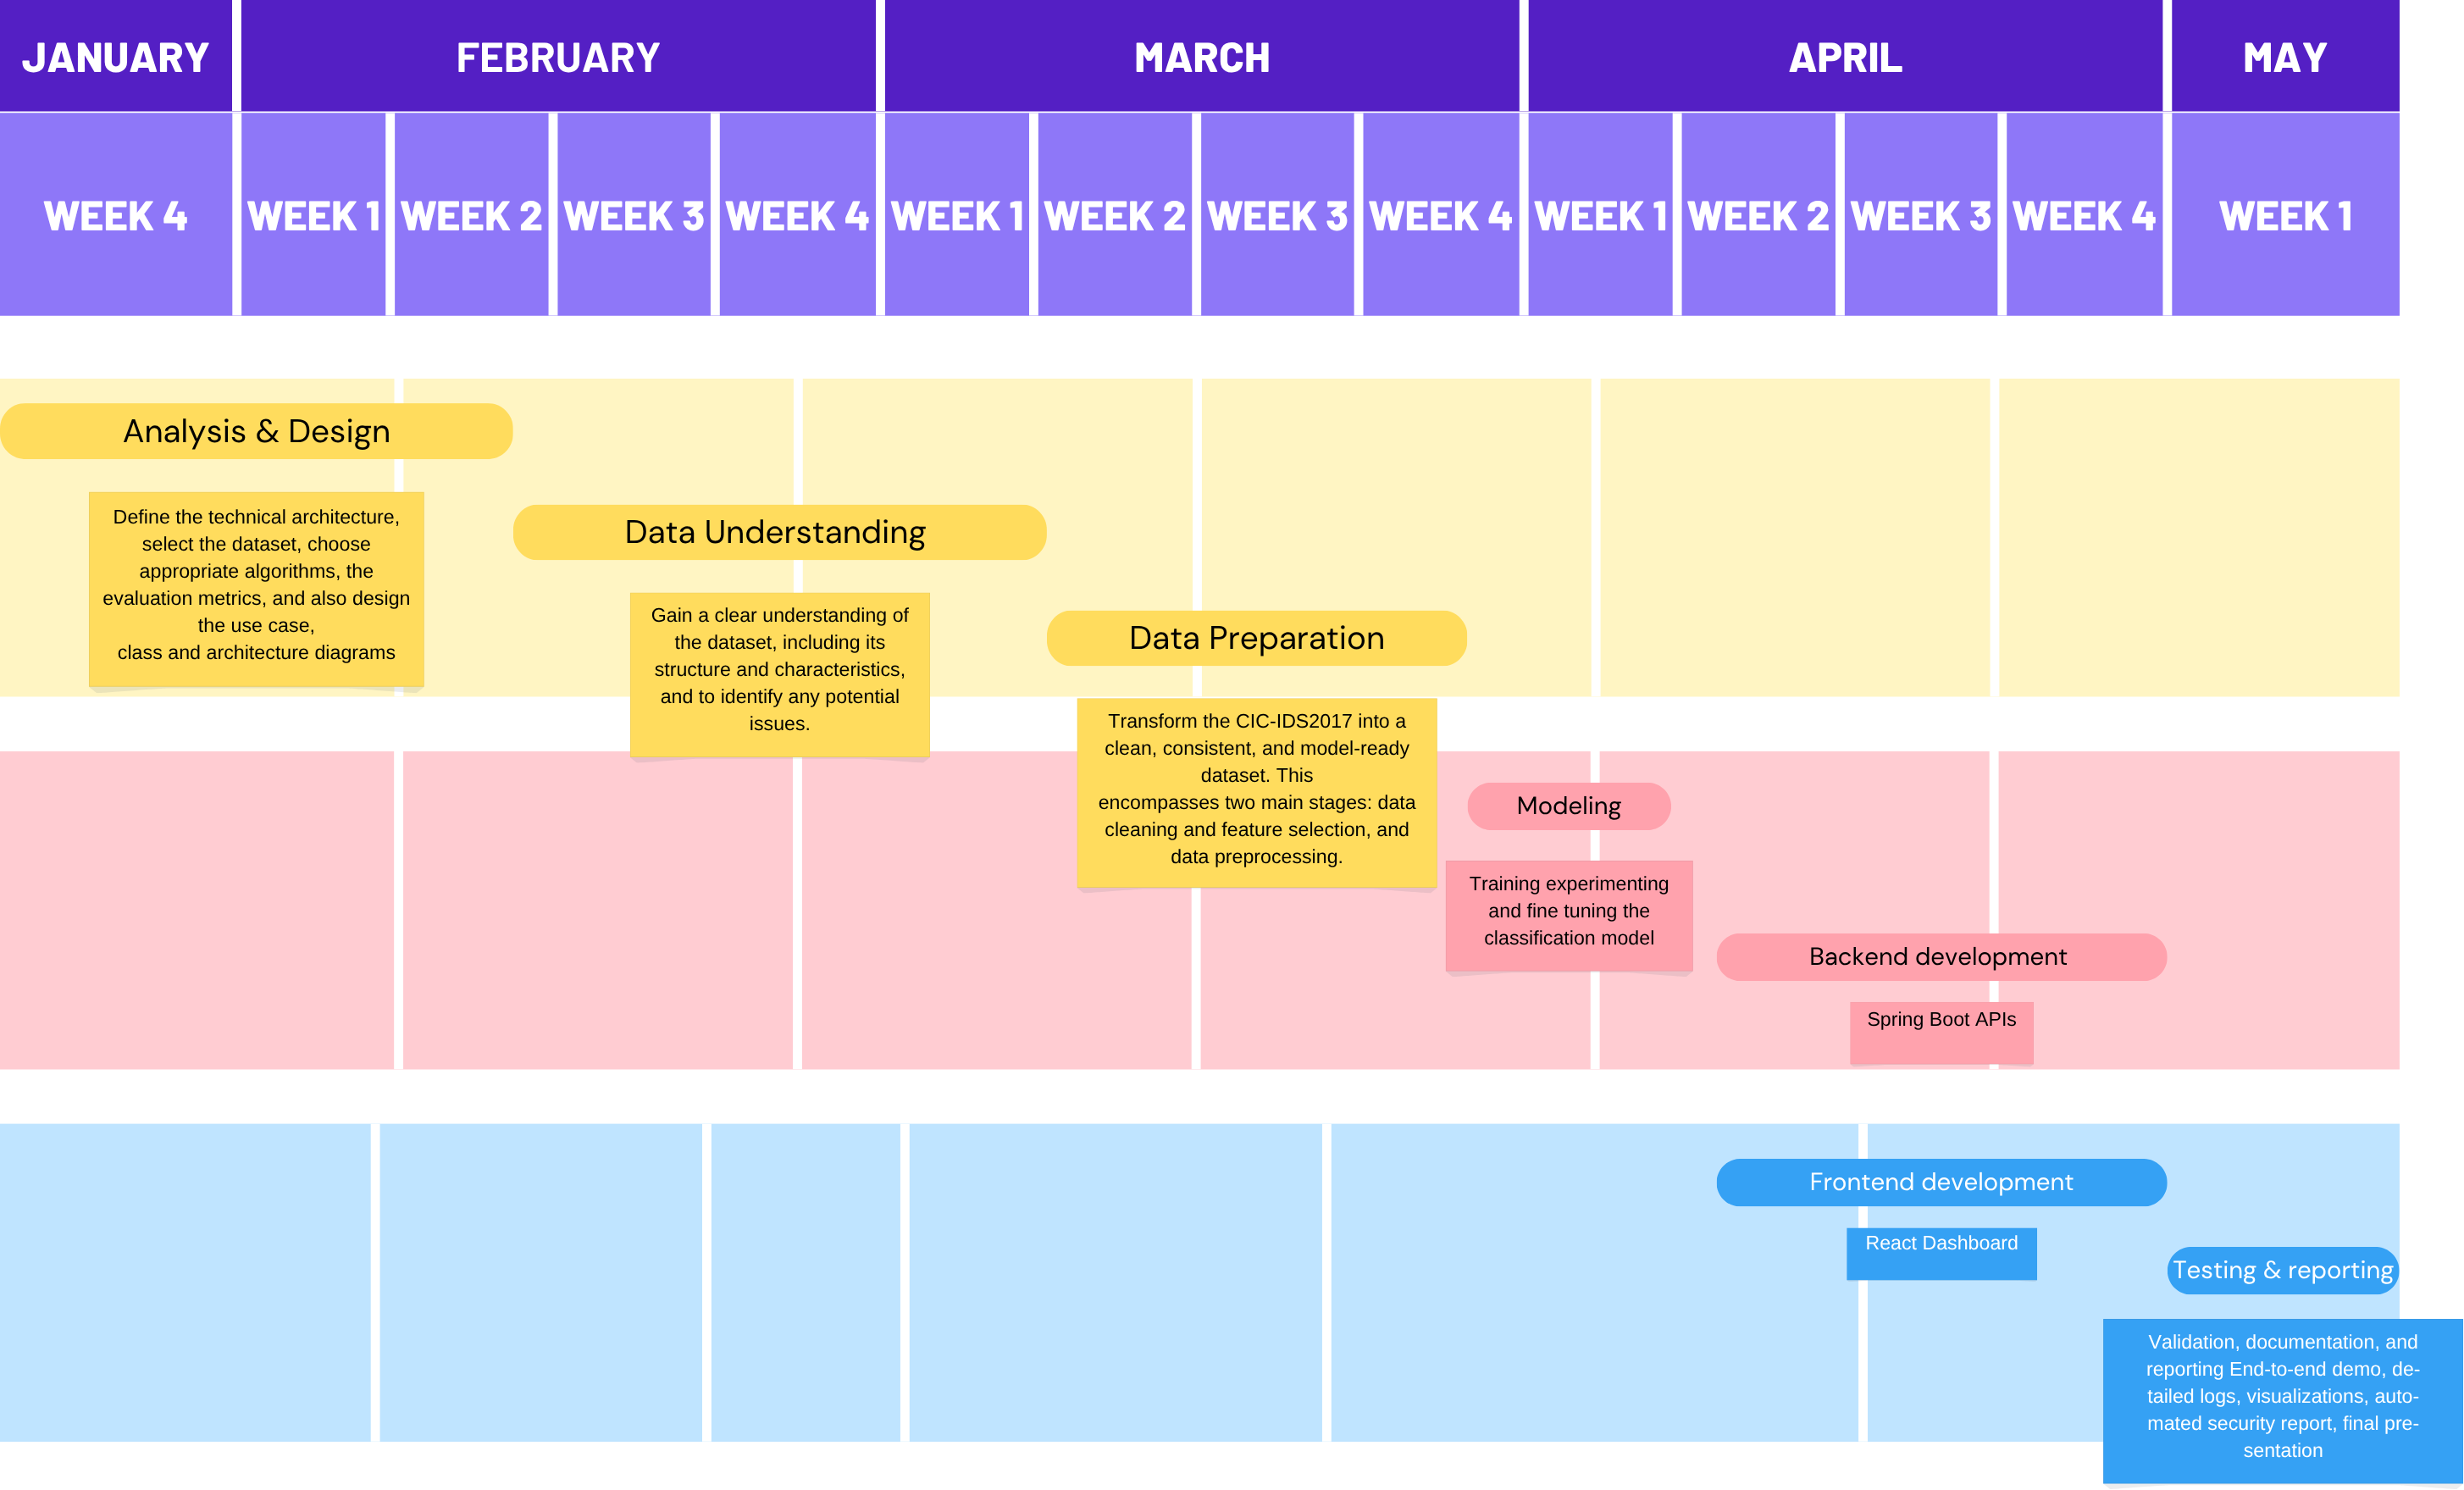
\includegraphics[width=1\columnwidth]{logos/pipeline.png}
    \caption{Project pipeline}
    \label{fig:pipeline}
\end{figure}

\section{Methodologies}
In this section, we present the methodologies that we use in this project, including the machine learning methodology CRISP-DM and the software development methodology UML language.
\newpage
\subsection{CRISP-DM}
The CRISP-DM (Cross-Industry Standard Process for Data Mining) methodology is a widely used framework for structuring machine learning projects. Figure~\ref{fig:crisp-dm} illustrates the six phases of this methodology and their relationships.

\begin{figure}[h!]
    \centering
    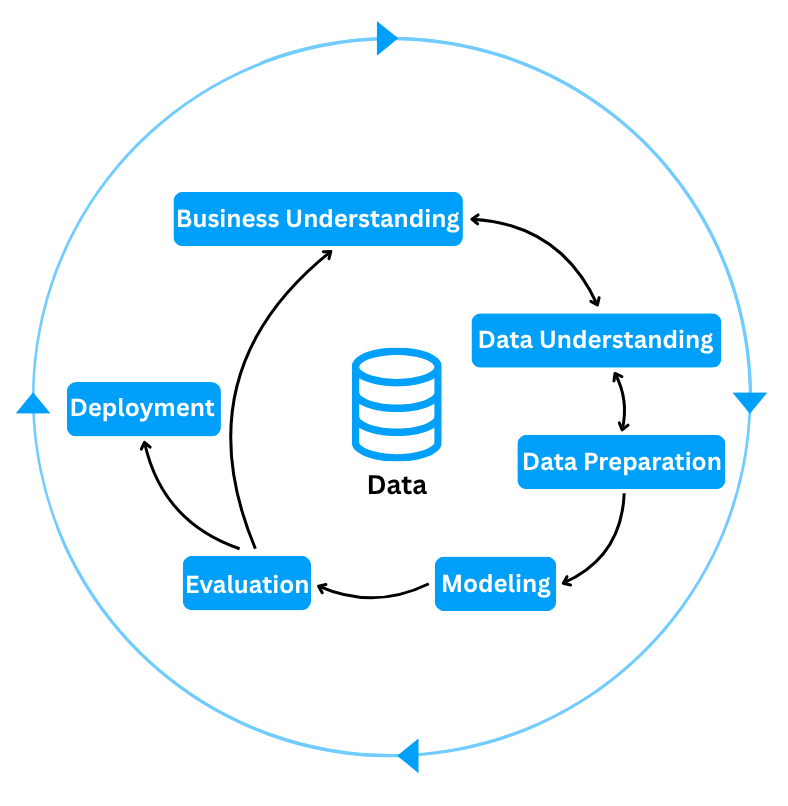
\includegraphics[width=0.6\columnwidth]{logos/CRISP-DM.png}
    \caption{CRISP-DM methodology}
    \label{fig:crisp-dm}
\end{figure}

\subsection{UML Language}
For the modeling of the software system, we use the UML (Unified Modeling Language) language it is a standardized modeling language that helps in specifying, visualizing, constructing, and documenting the artifacts of software systems using diagrams such as use case diagram, class diagram, and sequence diagram.

\begin{figure}[h!]
    \centering
    
\includegraphics[width=0.5\columnwidth]{logos/UML_logo.png}
    \caption{UML language \cite{UML}}
    \label{fig:uml}
\end{figure}

\newpage
\section{Conclusion}
In this chapter we introduce the host company ITXTREE, study existing network intrusion detection systems, discuss their shortcomings and finally present a solution. In the next chapter we specify the system requirements.

